\chapter{Perifer interaktion}
\label{PeriferInteratkion}
%
Skriv en hat
% 
\begin{itemize}
  \item Perifer interaktion - de to yderpunkter
  \item Opmærksomhed (perifer opmærksomhed)
  \item Hvorfor er det interesant at designe produkter, som kan reagere på perifer interaktion? (fordele og ulemper) 
  \item Inddrag at det er relativt nyt og ukendt at have produkter, som man kan interagere med perifert 
  \item Microgestures 
  \item Socialt acceptabelt 
  \item Hvordan har perifer interaktion ændret sig? (nu er det blevet skærmbaseret)
  \item Adfærdsændringer
  \item Relateret produkter  
  \item Baggrund/teori 
  \item Calm og Casual 
  \item Feedback 
\end{itemize}
%
Som nævnt tidligere er perifer interaktion ikke nyt. Vi gør det alle sammen, når vi i løbet af vores dagligdag foretager adskillige aktiviteter i vores perifere opmærksomhed, hvilket forudsætter at disse perifere interaktioner primært retter sig mod ikke-computer-relateret aktiviteter, \parencite[s. 1]{PDF:PeripheralInteraction}. 

%
\begin{figure}[H]
	\centering
	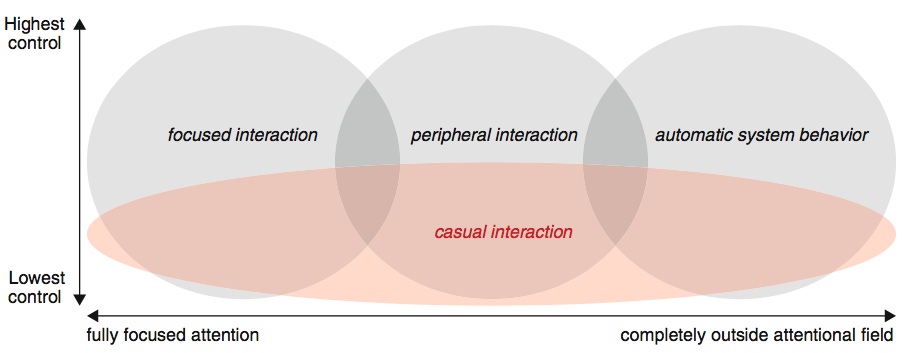
\includegraphics[resolution=300,width=\textwidth]{LevelsOfInteraction}
	\caption{ny \textcite[s. 118]{PDF:PeripheralInteraction}.}
	\label{fig:LevelsOfInteraction}
\end{figure}
\noindent
%